\subsection{Упражнение 1}

Пилообразный сигнал линейно нарастает от -1 до 1, а затем резко падает до -1 и повторяется.

\noindent Напишите класс, называемый SawtoothSignal, расширяющий signal и предоставляющий evaluate для оценки пилообразного сигнала.

\noindent Вычислите спектр пилообразного сигнала. Как соотносится его гармоническая структура с тругольными с прямоугольными сигналами?

Для создания пилообразного сигнала создадим класс SawtoothSignal. В методе класса evaluate опишем число циклов и c помощью библиотеки numpy разделим число циклов. unbias - смещает сигнал а normalize масштабирует его до заданной амплитуды.

\begin{lstlisting}[language=Python]
import thinkdsp

class SawtoothSignal(thinkdsp.Sinusoid):
  def evaluate(self, ts):
    cycles = self.freq * ts + self.offset / np.pi / 2
    frac, _ = np.modf(cycles)
    ys = thinkdsp.normalize(thinkdsp.unbias(frac), self.amp)
    return ys
\end{lstlisting}

\noindent Далее отобразим график пилообразного сигнала.

\begin{lstlisting}[language=Python]
saw = SawtoothSignal()
saw.plot()
saw_wave = saw.make_wave(duration=3, framerate=10000)
\end{lstlisting}

\begin{figure}[H]
	\begin{center}
		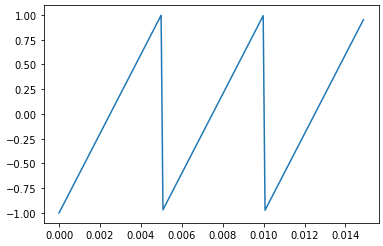
\includegraphics[scale=1]{fig/lab02/lab2_1.png}
		\caption{График пилообразного сигнала}
	\end{center}
\end{figure}

Мы действительно видим пилообразный сигнал. Далее сделаем экземпляр класса Wave для построения спектра сигнала.

\begin{lstlisting}[language=Python]
spectr = saw_wave.make_spectrum()
spectr.plot()
\end{lstlisting}

\begin{figure}[H]
	\begin{center}
		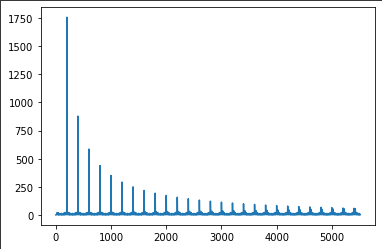
\includegraphics[scale=1]{fig/lab02/lab2_2.png}
		\caption{Спектр пилообразного сигнала}
	\end{center}
\end{figure}

Теперь сравним полученный спектр с треугольными и прямоугольными сигналами.

\begin{lstlisting}[language=Python]
triangle = TriangleSignal()
triangle.make_wave(duration=3, framerate=10000).make_spectrum().plot()
\end{lstlisting}

\begin{figure}[H]
	\begin{center}
		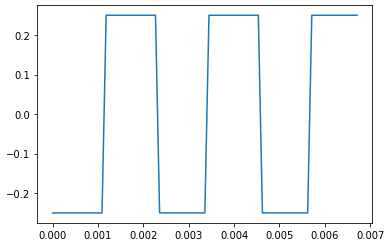
\includegraphics[scale=1]{fig/lab02/lab2_3.png}
		\caption{Спектр треугольного сигнала}
	\end{center}
\end{figure}

\begin{lstlisting}[language=Python]
square = SquareSignal()
square.make_wave(duration=3, framerate=10000).make_spectrum().plot()
\end{lstlisting}

\begin{figure}[H]
	\begin{center}
		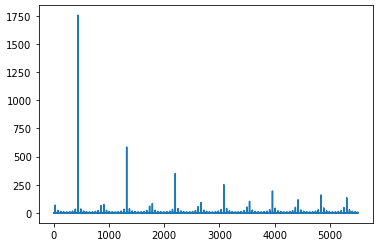
\includegraphics[scale=1]{fig/lab02/lab2_4.png}
		\caption{Спектр прямоугольного сигнала}
	\end{center}
\end{figure}

По сравнению с квадратным сигналом, пилообразный включает в себя четные и нечётные гармоники. Но оба сигнала снижают амплитуду обратно пропорциально частоте. По сравнению с изначальным сигналом, треугольный сигнал падает  1/f\^2 , а пилообразный  1/f .

\subsection{Упражнение 2}

Создайте прямугольный сигнал 1100 Гц и вычислите wave с выборками 10 000 кадров в секунду. Постройте спектр и убедитесь, что большинство гармоник "завёрнуты" из-за биений, слышно ли последствия этого при проигрывании?

\begin{lstlisting}[language=Python]
square = thinkdsp.SquareSignal(1100)
segment = square.make_wave(duration=1, framerate=10000)
spectr = segment.make_spectrum()
spectr.plot()
\end{lstlisting}

\begin{figure}[H]
	\begin{center}
		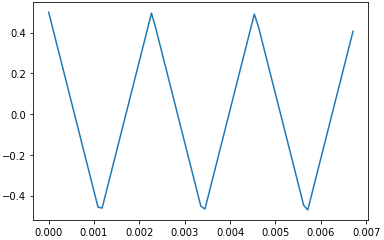
\includegraphics[scale=1]{fig/lab02/lab2_5.png}
		\caption{Спектр сигнала с биениями}
	\end{center}
\end{figure}

Из графика можно увидеть, что из-за фреймрейта, раввного 10.000 сигналы больших частот закольцовываются около 0Гц и 5Кгц - это называется биением. Когда мы слушаем получившийся звук - мы слышим основную частоту на 5КГц.


\subsection{Упражнение 3}

Возьмите объект спектра spectrum, и выведите первые несколько значений spectrum.fs, вы увидите, что частоты начинаются с нуля. Итак, «spectrum.hs[0]» — это величина компонента с частотой 0. Но что это значит?

\noindent Попробуйте этот эксперимент:

1. Сделать треугольный сигнал с частотой 440 и создать Волну длительностью 0,01 секунды. Постройте форму волны.

2. Создайте объект Spectrum и напечатайте spectrum.hs[0]. Каковы амплитуда и фаза этой составляющей?

3. Установите spectrum.hs[0] = 100. Создайте волну из модифицированного спектра и выведите ее. Как эта операция влияет на форму сигнала?

Создадим треугольный сигнал с частотой 440Hz и длительностью 0,01 сек, построим его график, распечатаем сигнал и распечатаем Spectrum.hs[0].


\begin{lstlisting}[language=Python]
signal = thinkdsp.TriangleSignal(440)
segment = signal.make_wave(0.01, framerate=10000)
segment.plot()
\end{lstlisting}

\begin{figure}[H]
	\begin{center}
		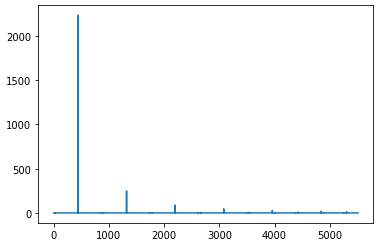
\includegraphics[scale=1]{fig/lab02/lab2_6.png}
		\caption{График сигнала}
	\end{center}
\end{figure}

Проверим что лежит в 0 элементе чисел спекторграммы.

\begin{lstlisting}[language=Python]
spectr = segment.make_spectrum()
spectr.hs[0]
\end{lstlisting}

\begin{lstlisting}
(1.375077994860476e-14+0j)
\end{lstlisting}
Видим комплексное число, с 0 мнимой частью. Сам элемент очень близок к нулю. Каждый элмент массива hs объекта Spectrum представялет собой комплексное число и соответствует частотоной компоненте: размах пропорционален амплитуде соответствующей компоненты, а угол - это фаза. Как видно из результатов выполнения кода, первый элемент массива hs - комплексное число, близкое к нулю, мнимая часть равна нулю.

\noindent Присвоим первый элемент 100 и посмотрим, что из этого выйдет.
\begin{lstlisting}[language=Python]
spectr.hs[0] = 100
spectr.make_wave().plot()
\end{lstlisting}

\begin{figure}[H]
	\begin{center}
		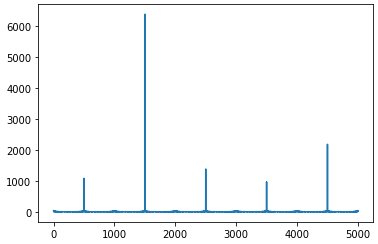
\includegraphics[scale=1]{fig/lab02/lab2_7.png}
		\caption{График сигнала с изменённым нулевым числом спекторграммы}
	\end{center}
\end{figure}

Как видно из полученного графика, сигнал сместился по вертикали. То есть первый элемент массив hs отвечает за смещение сигнали относительно вертикали. Если элемент близок или равен нулю, сигнал не смещенный.

\subsection{Упражнение 4}

Напишите функцию, которая принимает Spectrum в качестве параметра и модифицирует его, деля каждый элемент hs на соответствующую частоту из fs. Протестируйте свою функцию, используя один из файлов WAV в репозитории или любой объект Wave.

1. Рассчитайте спектр и начертите его.

2. Измените спектр, используя свою функцию, и снова начертите его.

3. Сделать волну из модифицированного Spectrum и прослушать ее. Как эта операция влияет на сигнал?


Исходя из последнего пункта первый элемент очень близок к нулю. Поэтому на него делить не надо, а то получим очень большие значения.

\begin{lstlisting}[language=Python]
def spec_div(spec):
  spec.hs[1:] /= spec.fs[1:]
  spec.hs[0] = 0
  spec.plot()

triangle = TriangleSignal()
wave = triangle.make_wave(duration=0.5, framerate=10000)
wave.make_audio()

spectr = wave.make_spectrum()
spectr.plot()
\end{lstlisting}

\begin{figure}[H]
	\begin{center}
		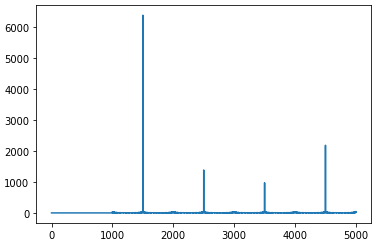
\includegraphics[scale=1]{fig/lab02/lab2_8.png}
		\caption{Спектр треугольного сигнала}
	\end{center}
\end{figure}

Применим написанную функцию.

\begin{lstlisting}[language=Python]
spec_div(spectr)
\end{lstlisting}

\begin{figure}[H]
	\begin{center}
		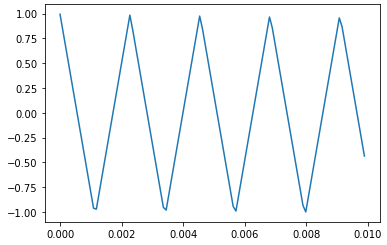
\includegraphics[scale=1]{fig/lab02/lab2_9.png}
		\caption{Спектр изменённого сигнала}
	\end{center}
\end{figure}

\begin{lstlisting}[language=Python]
spectr.make_wave().make_audio()
\end{lstlisting}

Видим. что ампилутуда очень поменялась, а частоты стоящие ближе к 0 Гц стали больше, чем следующие, что понятно.
Если сравнить полученные графики, можно сделать вывод, что функция действует как фильтр низких частот: частоты ослабляются на некоторую величину. Если сравнить две полученных звука на слух, то второй звучит более чисто, из-за отсутсвия низких часот, похож на звук синусоидального сигнала.

\subsection{Упражнение 5}

Треугольные и прямоугольные волны имеют только нечетные гармоники; пилообразная волна имеет как четные, так и нечетные гармоники. Гармоники прямоугольной и пилообразной волн затухают пропорционально $1/f$; гармоники треугольной волны затухают как $1/f^2$. Можете ли вы найти форму волны, в которой четные и нечетные гармоники затухают как $1/f^2$?

\noindent Подсказка: есть два способа подойти к этому: вы можете построить нужный сигнал путем сложения синусоид, или вы может начаться с сигнала, похожего на то, что вы хотите, и изменить его.


\noindent Не зря мы писали предыдущую функцию, поэтому возьмём пилообразный сигнал который имеет и четные и нечётные гармоники, а потом применим нашу функцию.

\begin{lstlisting}[language=Python]
saw_sign = SawtoothSignal(400)
saw_w = saw_sign.make_wave(duration=0.5, framerate=20000)
spectr = saw_w.make_spectrum()
spectr.plot()
decorate(xlabel='Frequency (Hz)')
\end{lstlisting}

\begin{figure}[H]
	\begin{center}
		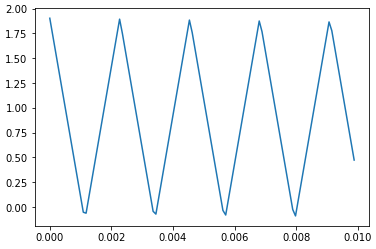
\includegraphics[scale=1]{fig/lab02/lab2_10.png}
		\caption{Спектр пилообразного сигнала}
	\end{center}
\end{figure}

Применим функцию для изменения амплитуды спада

\begin{lstlisting}[language=Python]
spec_div(spectr)
spectr.scale(400)
spectr.plot()
\end{lstlisting}

\begin{figure}[H]
	\begin{center}
		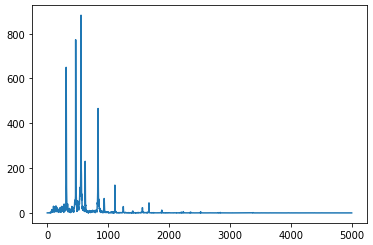
\includegraphics[scale=1]{fig/lab02/lab2_11.png}
		\caption{Спектр пилообразного сигнала после функции}
	\end{center}
\end{figure}

\begin{lstlisting}[language=Python]
spectr.make_wave().segment(duration=0.01).plot()
\end{lstlisting}

\begin{figure}[H]
	\begin{center}
		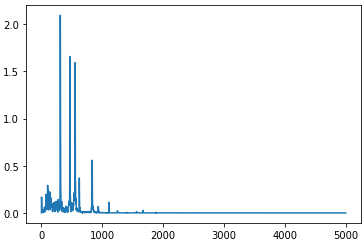
\includegraphics[scale=1]{fig/lab02/lab2_12.png}
		\caption{График сигнала}
	\end{center}
\end{figure}

Видно, что спектр спадает пропорционально квадрату частоты и при этом имеет четные и нечетные гармоники

\subsection{Вывод}

В ходе данной ладораторной работы были произведены различные действия с разными видами сигналов, а также были рассмотрены спектры и гармонические структуры и биения.